%!TEX encoding = UTF-8 Unicode
\documentclass[12pt]{scrartcl}
%\usepackage[applemac]{inputenc} % Mac-Umlaute direkt verwenden öäüß
%\usepackage[isolatin]{inputenc} % PC-Umlaute direkt verwenden 
\usepackage[utf8]{inputenc} % Unicode funktioniert unter Windows, Linux und Mac
\usepackage[T1]{fontenc}
\usepackage{times}
\usepackage[ngerman]{babel}
\usepackage{csquotes}
\usepackage[
backend=biber,
bibstyle=ieee,
citestyle=ieee
]{biblatex}
%\usepackage{ngerman}
\usepackage{graphicx}
\usepackage[hidelinks]{hyperref}\urlstyle{rm}
\usepackage{times}
\usepackage[scaled]{helvet}
\usepackage{a4wide}
\usepackage{rotating}
\usepackage{listings}\lstset{breaklines=true,breakatwhitespace=true,frame=leftline,captionpos=b,xleftmargin=6ex,tabsize=4,numbers=left,numberstyle=\ttfamily\footnotesize,basicstyle=\ttfamily\footnotesize}
\sloppy
\setlength{\parindent}{0em}
\setlength{\parskip}{1.2ex plus 0.5ex minus 0.5ex}
\pagestyle{plain}
\addbibresource{sem.bib}

\begin{document}

\newpage
\thispagestyle{empty}
\begin{center}\Large
Universität Hamburg \par
Fachbereich Informatik
\vfill
Seminararbeit
\vfill
{\Large\textsf{\textbf{Vergleich von IPSec und OpenVPN}}\par}
\vfill
von 
\par\bigskip
Mustafa Eris, Jim Martens, Benjamin Scholz \par
Betreuer: Hannes Federrath \par
%Matrikelnummern 6420323 \par
%Studiengang BSc. Informatik
\end{center}

\newpage
\section*{Zusammenfassung}


\newpage
\tableofcontents

\newpage
\section{Vorbemerkung}
Problem: VPN (Virtual Private Network) aufsetzen
Relevanz: sichere Kommunikation zwischen zwei privaten Netzwerken

\section{Grundlagen}
Was sind VPNs? Warum braucht man sie? Wozu werden sie verwendet?
Was ist das OSI-Referenzmodell? Wie ist es aufgebaut?
\section{IPSec}
\subsection{Entstehungsgeschichte}
IPSec ist unter der Aufsicht eines Komitees entstanden. Diese Vorgehensweise wurde dabei gezwungenermaßen auferlegt und erschwerte nach Ansicht vieler Mitwirkender die Arbeit erheblich.\cite{Ferguson2000}

Die Entstehungsweise führte dazu, dass IPSec unnötig kompliziert wurde. Die einen Mitglieder wollten die eine Lösung implementieren und andere plädierten für eine andere Lösung, was dazu führte, dass beide Lösungen implementiert wurden. Dies geht jedoch zu Lasten der Nutzbarkeit. Zu viele Optionen führen nicht nur zur Verwirrung und Komplizierung der Implementation von IPSec bei den Nutzern, es kann vor allem auch zu Sicherheitslücken führen. Experten bemängelten diese Komplexität.

Die erste Version von IPSec ist 1995 spezifiziert worden. Doch über die Jahre ist der Standard immer weiter entwickelt worden und so gibt es eine zweite Version aus 1998 und eine dritte aus 2005. Diese gelten zwar allgemein als V2 und V3, jedoch sind verschiedene Aspekte von IPSec in verschiedenen sogenannten ``Request for Comments"', kurz RFC, spezifiziert. So gibt es beispielsweise ein RFC, dass sich allgemein auf IPSec bezieht, aktuell RFC 4301 aus 2005, und es gibt beispielsweise ein RFC, dass sich auf die zu verwendenden Verschlüsselungsalgorithmen bezieht, aktuell RFC 7321 bereits aus 2014. So ist gewährleistet, dass IPSec weiterhin auf dem neuesten Stand gehalten werden kann, ohne dass man jedes mal die komplette Spezifikation überarbeiten muss.

Die folgenden RFCs sind für IPSec relevant:
\begin{itemize}
\item RFC 4301: Beschreibt den grundsätzlichen Aufbau von IPSec
\item RFC 4302: Beschreibt den Authentication Header (AH)
\item RFC 4303: Beschreibt Encapsulating Security Payload (ESP)
\item RFC 7321: Gibt vor welche Algorithmen für AH und ESP verwendet werden sollten
\item RFC 5996: Beschreibt das Internet Key Exchange Protocol Version 2 (IKEv2)
\item RFC 4307: Gibt vor welche Algorithmen für IKEv2 verwendet werden sollten
\item RFC 4308: Gibt Empfehlungen für Sammlungen von Algorithmen, die verwendet werden können
\end{itemize}
Es gibt noch viel mehr RFCs die man IPSec zuordnen kann, doch dies sind die wichtigsten. Im folgenden Abschnitt werden wir näher auf die technischen Aspekte von IPSec eingehen und die Themen der einzelnen RFCs näher betrachten.

\subsection{Technischer Aufbau}
\subsubsection{Tunnel Modus und Transport Modus}
IPSec kann in zwei verschiedenen Modi betrieben werden: Transport Modus oder Tunnel Modus. 

Beim Tunnel Modus werden die IP-Pakete in neue Pakete verpackt mit einem neuen Header. Dabei werden die Pakete jedoch von den einzelnen Gateways bearbeitet. Das heißt im Endeffekt, dass die Sicherheit nur von Gateway zu Gateway gewährleistet wird und nicht vom einem Ende zum anderen. Der Vorteil ist, dass der Endnutzer die Anwendung nicht merkt, da zum Beispiel der Router dies übernehmen kann. 

Im Transport Modus ist die Sicherheit vom einen zum anderen Ende gewährleistet. Dabei werden die eigentlichen IP-Pakete beibehalten und einige sicherheitsrelevante Felder hinzugefügt.
\subsubsection{Authentication Header}
Der Authentication Header, kurz AH, kann dazu verwendet werden, um die Authentizität und Integrität von Daten zu gewährleisten, und außerdem um Replay-Angriffe abzuwehren. Er muss im Gegensatz zur Alternative "`Encapsulating Security Payload"' jedoch nicht von IPSec Implementationen unterstützt werden.\footnote{RFC 4301 3.2.  How IPsec Works} Der Grund hierfür ist, dass ESP neben dem, was der AH leistet, zusätzlich noch die Vertraulichkeit der Pakete sicherstellt. Der Authentication Header wird dabei an die IP-Pakete angehängt und sieht wie folgt aus:

%\begin{figure}[htbp] 
%  \centering
%     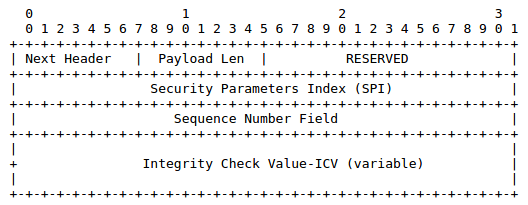
\includegraphics[width=0.7\textwidth]{AH-Aufbau.png}
%  \caption{Aufbau des Authentication Headers aus RFC 4302}
%  \label{AH-Aufbau}
%\end{figure}

Das 8 Bit lange Feld "`Next Header"' gibt an welche Art Nutzdaten nach dem AH folgen. Eine 4 bedeutet zum Beispiel IPv4 und eine 41 IPv6. Das 8 Bit lange Feld "`Payload Length"' gibt die Länge des AH in 4 Byte Worten - 2 an. Das 16 Bit lange Feld "`Reserved"' ist reserviert, damit man es in Zukunft nutzen kann, falls es benötigt wird. Das 32 Bit lange Feld "`Security Parameters Index"' (SPI) enthält die verwendete Security Association, die beim Versenden des Paketes verwendet wurde. Die Security Association beschreibt dabei, welche Sicherheitsdienste verwendet wurden, damit der Empfänger das Paket verarbeiten kann. Das 32 Bit lange Feld "`Sequence Number"' wird bei jedem versendeten Paket um 1 erhöht, um so Replay-Angriffe zu verhindern. Der Empfänger akzeptiert das Paket dabei nur, wenn die Sequence Number dabei in einem bestimmten Fenster liegt. Dieses Fenster ist daher vorhanden, da Pakete oft nicht in der selben Reihenfolge empfangen, wie sie versendet werden. Außerdem ist die Nummer mit einer MAC geschützt. Das heißt, wenn der Angreifer die Nummer ändert, dann stimmt der MAC nicht, und wenn er sie nicht ändert, dann fällt diese nicht mehr in das Fenster. Es gibt auch die Möglichkeit ein erweitertes 64 Bit langes Feld für die Sequence Number zu verwenden. 

Das Feld "`Integrity Check Value"' (ICV) enthält den MAC-Wert. Da dieser je nach verwendetem Algorithmus unterschiedlich lang ist, hat das Feld ebenfalls eine Variable Länge, dessen Beschränkung allerdings ist, dass es ein Vielfaches von 32 Bit sein muss, und dass der komplette AH ebenfalls ein vielfaches von 32 Bit bei IPv4 und ein vielfaches von 64 Bit bei IPv6 sein muss. Der MAC-Wert wird zur Überprüfung der Authentizität der Daten verwendet, das heißt es wird überprüft, ob das Paket auch tatsächlich vom Absender und nicht von einem Angreifer stammt.
\subsubsection{Encapsulating Security Payload}
Die Alternative zum AH ist "`Encapsulating Security Payload"', kurz ESP. Wie schon erwähnt muss ESP von IPSec-Implementationen unterstützt werden. 
ESP schützt auch wie AH die Integrität und Authentizität der Daten. Zusätzlich bietet es auch noch einen Schutz der Vertraulichkeit. Um dies zu erreichen können die Daten verschlüsselt werden. Der Aufbau von ESP ist wie folgt:
%Abbild Aufbau des ESP
Im Allgemeinen wird zwischen dem Header, der vor den Nutzdaten kommt, dem Trailer, welcher nach den Nutzdaten angelegt ist, und dem Feld zum Prüfen der Authentizität unterschieden. Das heißt beim ESP sind die Nutzdaten, wie der Name schon schließen lässt, von diesen Feldern umgeben.

Das 32 Bit lange Feld "`Security Parameters Index"' (SPI) wird genau wie beim AH verwendet. Das 32 Bit lange Feld "`Sequence Numbers"' ist ebenfalls sehr ähnlich zu dem entsprechenden Feld im AH, allerdings muss die Empfänger die Nummer ignorieren, wenn der Algorithmus zur Überprüfung der Integrität Null ist. Es gibt auch die Option zu einer Erweiterung zu einem 64 Bit langem Feld. Das Feld "`Payload Data"' hat eine variable Länge. Es enthält die Nutzdaten des Paketes. Das Feld "`Padding"' ist 0 bis 255 Bytes lang und kann zu verschiedenen Zwecken verwendet werden. Es gibt einige Verschlüsselungs-Algorithmen die nur Inhalte verschlüsseln können die ein Vielfaches einer bestimmten Byte-Zahl sind. Mit dem Padding-Feld können so die Nutzdaten aufgefüllt werden. Eine weitere Anwendungsmöglichkeit ist mit dem Feld die tatsächliche Länge für einen Angreifer zu verbergen, allerdings wird davon im RFC abgeraten, da dies nicht effektiv genug ist und das optionale Feld "`TFC Padding"' dafür bereits vorgesehen ist. Dieses Feld ist anders als das normale Padding-Feld nicht auf 255 Bytes limitiert und kann so einen Angreifer, der die Verkehrsdaten analysiert abwehren. Man kann das Feld im Transport-Modus jedoch nicht immer anwenden. 

Eine weitere Möglichkeit die Verkehrsdaten-Analyse zu verhindern ist dummy-Pakete zu versenden, die keinen nützlichen Inhalt haben, was aber nur für den Absender und Empfänger ersichtlich ist.

Das Feld "`Pad Length"' enthält die Länge des Padding-Feldes, jedoch nicht des TFC-Padding-Feldes, da dessen Länge in dem Payload Data-Feld gespeichert wird.%herausfinden warum genau
Das Feld "`Next Header"' ist 8 Bit lang. Es funktioniert ähnlich wie das entsprechende Feld des AH. Es wird benutzt um den Typ der Nutzdaten zu speichern. Wie schon beim AH gibt es zum Beispiel Werte für IPv4 und IPv6, aber zusätzlich gibt es beim ESP noch den Wert 59, welcher auf ein dummy-Paket hinweist. Das Feld "`Integrity Check Value"' hat eine variable Länge und enthält wie schon beim AH den Message Authentication Code, der benutzt wird um die Authentizität und Integrität der Nachricht zu prüfen. Der MAC wird dabei aus allen vorigen Feldern berechnet und wenn der Inhalt verschlüsselt wird, dann wird der MAC erst nach dem Verschlüsseln generiert. 

\subsubsection{Algorithmen}
In RFC 4835 ist festgehalten welche Algorithmen implementiert werden können, sollen oder müssen. Dabei sind die Algorithmen mit den Bewertungen must, must not, should, should not und may versehen. Zusätzlich gibt es zum Beispiel must-, was bedeutet, dass es zwar noch implementiert werden muss, aber wahrscheinlich bald zu should herabgestuft wird. Dabei wird unterschieden zwischen Verschlüsselungs-Algorithmen und Authentifizierungs-Algorithmen für ESP und Authentifizierungs-Algorithmen für AH.

Für ESP muss zur Zeit zur Verschlüsselung AES-CBC unterstützt werden. Hierbei werden die Felder Payload Data, Padding, TFC Padding, Pad Length und Next Header verschlüsselt. Im RFC 7321 steht außerdem, dass der Algorithmus Null unterstützt werden muss, was lediglich bedeutet, dass es auch möglich sein muss die Daten nicht zu verschlüsseln.

Die Algorithmen zum Authentifizieren sind bei AH und ESP gleich. Unterstützt werden muss HMAC-SHA1-96.\\
Es sind jeweils noch weitere Hinweise zu Algorithmen im RFC vorhanden, welche zum Beispiel unterstützt werden sollten oder auch nicht unterstützt werden dürfen. 
\subsubsection{Internet Key Exchange Version 2}
Es gibt bei IPSec eine ``Security Policy Database'' (SPD). Diese legt fest welche Verfahren angewendet werden dürfen, das heißt hier wird festgelegt welche Security Associations erstellt werden dürfen. Die Security Associations (SA) werden wiederum in einer eigenen Datenbank gespeichert, also in einer SAD. Die SA enthalten unter anderem auch die verwendeten Schlüssel.

Die SPD wird üblicherweise per Hand eingerichtet, da diese eher statisch ist und man während der Kommunikation keine Einträge vornehmen muss. Für die SAD wird üblicherweise IKEv2 verwendet, welches die SAs automatisch verwaltet.

Zunächst wird eine Prozedur durchlaufen, um eine Verbindung zwischen den Kommunizierenden herzustellen. Die einzelnen Schritte bestehen immer aus einer Nachricht des Senders und einer Nachricht des Empfängers. Der erste Austausch wird IKE\_SA\_INIT genannt. Hierbei werden zunächst Daten ausgetauscht, um zu vereinbaren wie die Verbindung hergestellt wird, also z.B. welche Algorithmen verwendet werden. Dazu schickt der Initiator dem Empfänger Vorschläge wie die Verbindung aussehen soll und der Empfänger bestätigt dann seine Auswahl. Außerdem werden Diffie-Hellman Werte und Noncen ausgetauscht. Anhand von diesen Werten und der Noncen wird SKEYSEED generiert. Mit Hilfe dieses SKEYSEEDs werden nun mehrere Schlüssel erstellt, die zum Verschlüsseln und Authentifizieren nachfolgender Kommunikation verwendet werden. Der nächste Austausch wird IKE\_AUTH genannt. Dieser Austausch ist mit den vorher generierten Schlüssel geschützt und nun können sich die Kommunizierenden, ebenfalls anhand der vorher generierten Schlüssel, authentifizieren. Nun wird eine SA ausgemacht, die letztendlich auch in die SAD eingetragen wird, also letztendlich genutzt wird um den später die eigentliche Datenkommunikation zu regeln.
Nachfolgende Kommunikation bezüglich IKE wird CREATE CHILD SA genannt und kann dazu genutzt werden um weitere SAs zu vereinbaren. Es gibt außerdem noch INFORMATIONAL, welches z.B. für Fehlermeldungen von IKEv2 und ähnliches genutzt wird.
%%%%%%%%%%%%%%%%%%%%%%%%%%%%%%%%%%%%%%%%%%%%%%%%%%%%%%%%%%%%%%%%%%%%%
\section{OpenVPN}
%\input{VPN}
Was ist OpenVPN? Wer ist dafür verantwortlich? Wie funktioniert es?
\subsection{Was ist ein VPN?}
Man stellt sich unter einem Netzwerk immer Verbindungen zwischen einzelnen Computern in Form von Verkabelungen vor. Ein VPN verbindet hingegen Rechner oder ganze Netzwerke über bereits vorhandene Netzwerke hinweg.

Virtuelle Private Netzwerke (VPN) erlauben eine sichere, stabile und preisgünstige Kommunikation über das Internet. Mit ihrer Hilfe können verteilte Unternehmensnetze verbunden werden oder Außendienstmitarbeiter auf Ressourcen und Daten in dem Unternehmensnetz zugreifen. Sie bieten eine kostengünstige und sichere Anbindung von Filialen an eine Zentrale und erlauben den Einsatz von Telearbeitsplätzen, bei denen die Angestellten ihre Arbeit zu Hause erledigen.

\subsection{Was ist ein OpenVPN?}

Open VPN ist eine VPN-Lösung, die unter Linux, Windows und vielen weiteren Betriebssystemen eingesetzt werden kann.
Open VPN ist eine freie Software und steht unter der GPL ( GNU General Public License ).

\subsection{Verschlüsselung bei OpenVPN}

OpenVPN benutzt zur Authentifizierung und Verschlüsselung der Daten kryptografische Verfahren auf Basis von TLS (Transport Layer Security). TLS ist ein Verschlüsselungsprotokoll zur Datenübertragung und der Nachfolger vom bekannteren SSL (Secure Sockets Layer).Die meisten Internetbrowser unterstützen TLS-Verbindungen. Dieses Protokoll wird im Internet u.a. zum Aufbau von sicheren Verbindungen  (HTTPS-Verbindungen) bei Banken oder Shopsystemen  eingesetzt. Daran erkennt man , dass dies allgemein anerkannte und vor allem auch ausgereifte  Standardverfahren ist.

\section{Vergleich von IPSec mit OpenVPN}

In den vorangegangenen Abschnitten wurden IPSec und OpenVPN vorgestellt. In diesem Abschnitt widmen wir uns dem Vergleich der beiden. Damit ein solcher Vergleich jedoch sinnvoll stattfinden kann, muss im Voraus klar sein, was verglichen wird. Wir benötigen daher Kriterien. Im Folgenden werden die Kriterien erarbeitet und erläutert, warum wir das jeweilige Kriterium für wichtig befinden.

\subsection{Kriterien}
Ein Hauptziel von VPNs ist die sichere Kommunikation zwischen zwei privaten Netzen. In dem Ziel selber steckt daher bereits Sicherheit als Anforderung. Es muss sichergestellt sein, dass Nachrichten von einem Netz zum anderen gelangen, ohne dass sie unterwegs in irgendeiner Weise beeinträchtigt werden. Aus diesem Grund ist natürlich von großem Interesse, wie sicher IPSec bzw. OpenVPN sind und weitergehend, ob eine der beiden Varianten sicherer ist als die andere.

Aus was setzt sich die Sicherheit jedoch zusammen? Zur Sicherheit gehören einerseits die Schutzziele in der IT-Sicherheit: Vertraulichkeit, Integrität, Verfügbarkeit. Andererseits gehören aber auch das Vorhandensein von Sicherheitslücken zur Sicherheit. Denn was nutzt ein theoretisch sicheres Verfahren, wenn es in der Implementation reihenweise Sicherheitslücken gibt?

Allerdings ist es nicht wirklich gangbar IPSec und OpenVPN anhand von Sicherheitslücken zu vergleichen, denn während IPSec ein Standard ist\cite{Kent2005}, handelt es sich bei OpenVPN um eine konkrete Implementation eines SSL/TLS-basierten VPNs\cite{Kotuliak2011}. Daher haben wir uns dagegen entschieden Sicherheitslücken in den Vergleich mit einzubeziehen.

Allerdings sind wir damit noch nicht am Ende unserer Kriterien angelangt. Aus dem Schutzziel der Verfügbarkeit lässt sich die Performance als Kriterium ableiten. Schließlich interessiert es neben der Sicherheit auch, wie schnell die Nachrichten von A nach B kommen. Was konkrete Werte bei einem Performancevergleich angeht, verweisen wir auf einen solchen Vergleich von 2011, welcher im Rahmen der ICETA Konferenz von Kotuliak\cite{Kotuliak2011} unternommen wurde.

Ein weiteres Kriterium ist die Kompatibilität zwischen Lösungen unterschiedlicher Hersteller. Dies liegt darin begründet, dass es aus Gründen der Sicherheit sinnvoll ist, Hardware unterschiedlicher Hersteller zu benutzen, da somit Sicherheitslücken bei einem Hersteller sich nicht auf das gesamte Netzwerk auswirken. Dies ist jedoch nur möglich, wenn die Implementationen der verschiedenen Hersteller zueinander kompatibel sind. In der Hinsicht hat auch Kompatibilität etwas mit Sicherheit zu tun.

Wir haben die Kriterien in dem obigen Abschnitt herausgearbeitet. Zusammengefasst sind es: Vertraulichkeit, Integrität, Verfügbarkeit, Performance und Kompatibilität.

\subsection{Vertraulichkeit}
Wir beginnen den Vergleich mit der Vertraulichkeit. Interessant sind da die unterstützten Verschlüsselungsalgorithmen und die maximalen Schlüssellängen der Algorithmen.

Im Abschnitt über IPSec wurde bereits eingeführt, dass IPSec grundlegend zwei Mechanismen unterstützt: ESP\footnote{Encapsulated Security Payload} und AH\footnote{Authentication Header}. Das Schutzziel der Vertraulichkeit wird dabei nur von ESP gewährleistet, weswegen wir AH beim Vergleich bzgl. der Vertraulichkeit ignorieren.

OpenVPN ist eine Implementation eines TLS-basierten VPNs. Die Verschlüsselung wird hierbei von dem TLS-Protokoll übernommen. Deswegen werden wir in diesem Punkt IPSec mit TLS vergleichen.

Für jedes Verschlüsselungsverfahren wird ein Schlüssel benötigt. Daher werden wir uns zunächst die verwendeten Verfahren zum Schlüsselaustausch ansehen. IPSec verwendet meistens Diffie-Hellman, unterstützt aber auch KINK\footnote{Auf Kerberos basierendes Protokoll, dass Schlüsselaustausch- und Authentifizierungsmechanismen bereitstellt. Es wurde noch nicht standardisiert\cite{Alshamsi2005}.}. TLS unterstützt mehrere Verfahren. In diesem Paper beschränken wir uns auf zwei davon: RSA und DH\footnote{Diffie-Hellman}\cite{Alshamsi2005}. %Im Falle von RSA sendet der Client den sogenannten \texttt{pre\_master\_secret}, nachdem dieser mit dem öffentlichen Schlüssel des Servers verschlüsselt wurde. Anhand dieses Wertes kann der Server nun das \texttt{master\_secret} errechnen, womit der Sitzungsschlüssel erzeugt wird. Der Client tut dies ebenfalls.

%Bei DH tauschen Client und Server die öffentlichen DH-Werte aus und erzeugen den \texttt{pre\_master\_secret} unabhängig voneinander. 

Es ist ersichtlich, dass IPSec und TLS DH unterstützen. Zusätzlich unterstützt IPSec KINK und TLS RSA. Ein wirklicher Vor- oder Nachteil kann in diesem Fall weder IPSec noch TLS zugesprochen werden. Wenn wir die Verbreitung von KINK bzw. RSA vergleichen, dann liegt RSA vorne, da es seit langem standardisiert ist und es etliche Implementationen gibt.

Ein weiterer Punkt bei der Vertraulichkeit ist die Authentifizierungsmethode. IPSec unterstützt lediglich die gegenseitige Authentifizierung. TLS hingegen unterstützt eine reine Server-Authentifizierung, eine gegenseitige Authentifizierung, die auch Client-Authentifizierung genannt wird, und eine anonyme Authentifizierung, bei der nichts authentifiziert wird.\cite{Alshamsi2005}

Bei den Authentifizierungsalgorithmen hat jedoch IPSec einen Vorteil, denn es wird sowohl die Nutzung einer digitalen Signatur als auch die Verwendung eines Algorithmus, der auf einem geheimen Schlüssel basiert, ermöglicht. TLS benötigt hingegen zwangsweise eine digitale Signatur. Sollten alle Algorithmen mit digitaler Signatur ausfallen, kann IPSec weiterhin implementiert werden, TLS jedoch nicht.\cite{Alshamsi2005}

Zusammenfassend kann für den Bereich der Vertraulichkeit gesagt werden, dass sowohl IPSec als auch TLS hinreichende Vertraulichkeit bieten.

\subsection{Integrität}
Neben der Vertraulichkeit ist auch die Integrität wichtig. Daher werden wir im folgenden Abschnitt vergleichen, welche Methoden von IPSec und OpenVPN zur Wahrung der Integrität verwendet werden.

Analog zur Vertraulichkeit wird auch hier nicht direkt OpenVPN verglichen, sondern TLS, da dieses zuständig dafür ist.

Als Authentifizierungsverfahren zur Überprüfung der Integrität werden von beiden Message Authentication Codes (kurz: MACs) verwendet. Bei MACs hängt es von dem verwendeten Hashverfahren an, ob die Integrität zuverlässig überprüft werden kann. Sowohl IPSec als auch TLS erfordern die Implementation von HMAC-SHA-1 und HMAC-MD5. HMAC ist eine kryptographische Hashfunktion, die einen geheimen Schlüssel erfordert. Die Sicherheit bzw. Stärke des Algorithmus hängt dabei von der Länge des Schlüssels und des Outputs ab.\cite{Alshamsi2005}

Als Fazit für die Integrität kann gelten, dass es keine wirklichen Unterschiede zwischen IPSec und TLS in diesem Bereich gibt.

\subsection{Verfügbarkeit}
Das dritte Schutzziel ist Verfügbarkeit. Traditionell fallen Dinge wie DDOS-Angriffe\footnote{Distributed-Denial-of-Service-Angriffe} unter dieses Schutzziel bzw. beeinträchtigen es. In unserem Zusammenhang ist die Durchlässigkeit bei Firewalls von Interesse, also ob ein VPN durch eine der beiden Technologien gezielt geblockt werden kann. Auch die Verbreitung spielt eine Rolle, denn eine weit verbreitete Technologie macht es intuitiv gesehen erst einmal "`einfacher"' eine Verbindung zwischen zwei Netzen aufzubauen.

Beginnen wir bei Firewalls. Dort gilt, dass IPSec in geringem Maße im Nachteil ist, da es feste Protokolle und Ports benötigt. Ein gezieltes Blocken von IPSec-basierten VPNs ist daher praktikabel. Im Vergleich dazu kann OpenVPN auf jedem Port mit UDP oder TCP laufen. Um restriktive Firewalls zu überwinden, kann der Port 443 und TCP benutzt werden. Dadurch sieht der Traffic von OpenVPN wie normaler HTTPS-Traffic aus und kann nicht gezielt gefiltert werden.\cite{ivpn.net}

Bei der Verbreitung hat IPSec wiederum einen leichten Vorsprung, denn die meisten Betriebssysteme unterstützen es nativ. Für OpenVPN muss hingegen jeweils ein Client installiert werden. Die Form des Client unterscheidet sich je nach Betriebssystem und ist in den meisten Fällen innerhalb von 5 Minuten erledigt.\cite{ivpn.net}

Für die Verwendung hinter hochrestriktiven Firewalls ist OpenVPN im Vorteil, da es die zu 99\% immer offenen Ports 80 und 443 mitbenutzen kann und somit nicht von normalem Browsertraffic zu unterscheiden ist. Bei allen Nutzungsszenarien spielt es jedoch keine Rolle, ob IPSec oder OpenVPN eingesetzt werden.

\subsection{Performance}
Nachdem wir IPSec und OpenVPN bezüglich der Schutzziele verglichen haben, widmen wir uns jetzt der Performance.

%TODO Vergleich Performance

\subsection{Kompatibilität}
Abschließend gehen wir auf die Kompatibilität der Implementationen verschiedener Hersteller untereinander ein. Uns war es nicht möglich eigene Vergleiche hinsichtlich der Kompatibilität durchzuführen, daher werden wir nur oberflächlich darauf eingehen.

OpenVPN benutzt TLS und dieses Protokoll ist seit langem erprobt und von einer Vielzahl an Herstellern implementiert. Obgleich es mit Heartbleed eine Sicherheitslücke in der bekannten Implementation OpenSSL gab, tut das der Kompatibilität keinen Abbruch. Es ist demnach vollkommen egal welche Hardware und welche Software verwendet wird, denn TLS wird mittlerweile in allen gängigen Systemen nativ unterstützt.

Bei IPSec sieht das anders aus. Zwar ist auch IPSec standardisiert, ebenso wie TLS, aber der Umfang der RFCs macht ein Verständnis relativ schwer. Daraus ist auch zu begründen, warum es zu Beginn kaum untereinander kompatible Lösungen gab\cite{Alshamsi2005}. Mittlerweile ist der Standard jedoch älter und auf breiterer Schicht umgesetzt, sodass es zwar noch Unterschiede zwischen TLS und IPSec gibt, diese jedoch nicht mehr ins Gewicht fallen.

Bezüglich der Kompatibilität kommen wir zu dem Fazit, dass IPSec noch im Vergleich zu TLS aufholen muss, allerdings bereits viele der anfänglichen Kompatibilitätsprobleme überwunden hat.

\section{Schlussbemerkungen}
Ausblick: (weitere) Vereinfachung von IPSec?, unterschiedliche Ansätze, Vor- und Nachteile bei beiden

%%%%%%%%%%%%%%%%%%%%%%%%%%%%%%%%%%%%%%%%%%%%%%%%%%%%%%%%%%%%%%%%%%%%%%
\newpage

\printbibliography
\addcontentsline{toc}{section}{Literaturverzeichnis}


%%%%%%%%%%%%%%%%%%%%%%%%%%%%%%%%%%%%%%%%%%%%%%%%%%%%%%%%%%%%%%%%%%%%%%
\newpage
\addcontentsline{toc}{section}{Anhang}

\end{document}
